\chapter{Empirical Study}
\label{chapter7}

In our final chapter we will suplement our ivestigation of the w-structures with an Empirical Study. This goal of this study if two-fold. Firstly to verify our theoretical claims on the correctness and running of the w-diameter algorithm we developed. This will be done by implementing and testing them. The second goal and most important goal of the empirical study is to analyse w-structes in contour trees of real life data sets using the algorithms we've implemented. We will then conclude the chapter with a discussion on the future directions this study can take.

\section{Datasets Overview}

Talk about the data sets we used. Mountain ranges taken from Canada.

\section{W-detector Algorithms}

We outlined how the algorithms are imeplemented in chapter 3. Here we will talk about testing correctness and running time.

To run tests we had to generate random height trees.

Tests correctness by using the 2xBSF algorihtm for groups truth. Easiest and most reliable. Generate a bunch of trees and check results. We test this many trees and DP had the same results, 2xBSF was always within two of the actual w-diameter. This is completely in line with what we expected.

Testing running by running on random trees in the range 5K-200K. Five different trees per mark averaged out.

\begin{figure}%
    \centering
    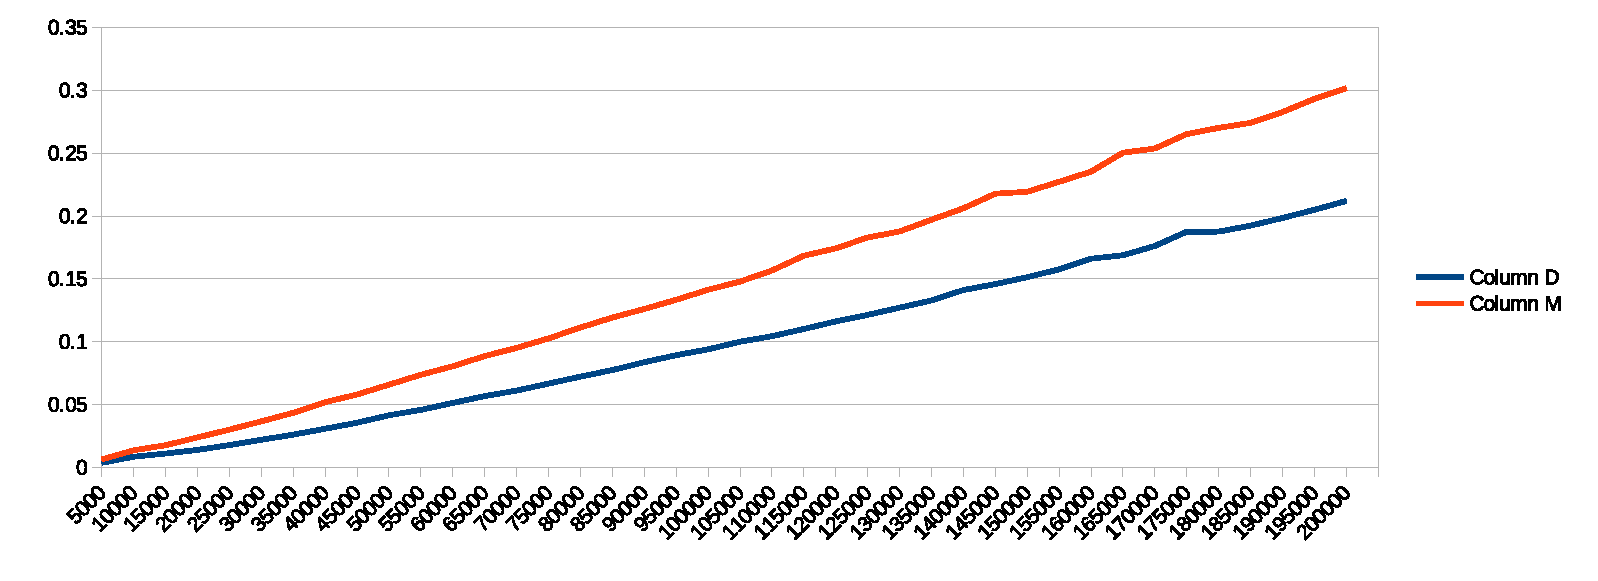
\includegraphics[center, scale=0.6 ]{./images/running-time-new.eps}
    \caption{Running time of 2xBFS (blue) and DP (red) on randomly generated trees. }%
    \label{fig:case1.1}%
\end{figure}

Bot algorithm appear to be linear on this scale and these trees. These begins to confirm the suspisions we had the DP is not quadratic in practice.

Here is the performance on the data sets we have.

\begin{center}
\begin{tabular}{l*{6}{c}r}
Dataset             & Vertices          & 2xBFS          & DP            & Factor \\
\hline
vanc                & 378               & 0.000254	& 0.000477      & 1.88 \\
vancouverNE         & 4851              & 0.003125	& 0.006393      & 2.05 \\
vancouverNW         & 4900              & 0.003165	& 0.006536      & 2.07 \\
vancouverSE         & 4950              & 0.002927	& 0.008382      & 2.86 \\
vancouverSW         & 5000              & 0.003119	& 0.006285      & 2.02 \\
vancouverSWNE       & 1250              & 0.000784	& 0.001408      & 1.80 \\
vancouverSWNW       & 1250              & 0.000862	& 0.001490      & 1.73 \\
vancouverSWSE       & 1275              & 0.000815	& 0.001651      & 2.03 \\
vancouverSWSW       & 1225              & 0.000814	& 0.001412      & 1.73 \\
icefield            & 57600             & 0.040002  & 0.070194      & 1.75 \\
pukaskwa            & 881600            & 0.551351  & 0.973880      & 1.76 \\
gtopo30w020n40      & 28800000          & -1        & -1            & -1 \\

\end{tabular}
\end{center}

As we can see the results are again consistent with what we had with the random data sets.


\section {Dataset w-diameter analysis}

Here is the epic table for the analysis of the datasets. Fix it it's wrong!

\begin{center}
\begin{tabular}{l*{6}{c}r}
Dataset             & Vectices  & 2BFS  & DP    & NBFS  & Diameter  & Iterations\\
\hline
vanc                & 378       & 2     & 2     & 2     & 311       & 2  \\
vancouverNE         & 4851      & 4     & 5     & 5     & 1338      & 5  \\
vancouverNW         & 4900      & 5     & 5     & 5     & 1456      & 5  \\
vancouverSE         & 4950      & 6     & 6     & 6     & 1306      & 5  \\
vancouverSW         & 5000      & 4     & 4     & 4     & 1977      & 4  \\
vancouverSWNE       & 1250      & 5     & 5     & 5     & 423       & 4  \\
vancouverSWNW       & 1250      & 3     & 3     & 3     & 712       & 3  \\
vancouverSWSE       & 1275      & 3     & 3     & 3     & 759       & 3  \\
vancouverSWSW       & 1225      & 2     & 2     & 2     & 845       & 3  \\
icefield            & 57600     & 7     & 7     & 7     & 12280     & 6  \\
pukaskwa            & 881600    & 180   & 182   & N/A   & 374866    & 94 \\
gtopo30w020n40      & 28800000  & 8     & 10    & N/A   & 15766966  & 8  \\

\end{tabular}
\end{center}

We can observe the following things:

\begin{itemize}
  \item Things and stuff1
      \item The w-diameter of a tree is a much better upper bound on the algorithm.
    \item The w-diameter can severely prevent logarithmic collapse.
    \item The w-diameter becomes prevalent in random samples of randomly generated tree. Therefore the law of large number will affect it.
\end{itemize}


\section{Generating W-Structures Manually}

We can generate them via ridges and valleys.


\section{Future Work}

Can be obtain the w-diameter from raw data?

Can we generate them in other ways?




% In this chapter we will study the w-structures empirically by implementing the algorithms that we can developed in Chapter \ref{chapter2} and using them to analyse real world data sets. The reason for studying them in practise is to learn more about them and explore how exactly they slow down computation. To accomplish this we will set two primary objectives. Firstly to correlate the iterations needed to collapse the contour tree in the merge phase of the algorithm with its w-diameter. This aims to give strength to the hypothesis that the w-structures do slow down computation in practise. Secondly to demonstrate that w-structures are found in real world data and do appear more abundantly as the size of datasets increases.
%
% In addition to out primary objectives there are some additional topics, related to the empirical study, that will be explored
%
% \begin{itemize}
%     \item Description the implementation of all used algorithms.
%     \item Demonstration of the running time of the implementations of the algorithms.
%     \item Correlating iterations for collapse with w-diameter of randomly generated tree.
%     \item Determining the smallest 2-dimensional grid dataset that exhibits a w-structure.
%     \item Discussion on the kinds of structures in raw data that produce w-structures in the contour trees.
%     \item Discussion on whether it is possible to determine the w-diameter of a datasets without computing it's contour tree beforehand.
%     %\item Exploring the statistical distribution of w-structures in randomly generated trees.
% \end{itemize}

%The first step to overcoming a problem is to learn about it. We .
%As a result of this study we will be able to shed light on the practical obstacles that the w-structures pose.

% For the purpose of the empirical study we implemented all three w-diameter algorithms we developed in the previous chapter. Those are the brute force algorithm, the 2xBFS and DP algorithms. In order to produce the contour trees of real life data sets we also implemented the serial version of the contour tree algorithm that is based directly on \cite{carr-masters}. To test our implementations for correctness we required the generations of more data sets than we had. This is why we have also written three small utility programs. One generates randomly populated data grids of size $n \times m$, the second generates random trees on $n$ vertices and lastly one that generates all $n \times m$ permutations of data grids populated with the numbers from $1$ to $n \times m$.  All algorithms were implemented in C++ and all algorithms are serial.
%
% The first algorithm that we implemented was the algorithm for computing the contour tree. To keep the implementation of this algorithm straightforward we have opted for working with two dimensional data sets only. To ensure the correctness of the implementation we have ran the code against code provided by Dr. Hamish Carr that implements the same algorithm. We have found that the two implementations produce the same output for all data sets we have tested - both from real data and random data.
%
% For the brute force algorithm and the 2xBFS algorithms we based our implementation entirely on the pseudocode provided in the previous chapter. The source code for those can be found in the appendix. For the DP algorithm we had to implemented a bottom up approach because the recursive one we suggested in the previous chapter was not efficient enough for large data sets. To adapt the algorithm to a bottom approach we firstly ran a standard Breadth First Search from a node in the tree. With it we computed the leaves, 1st order leaves, 2nd order leaves and so on. After this we extracted all of the code that was used in the backtracking phase of the Depth First Search and applied it first to all leaves, than 1st order leaves and so on. This ensured that all children of a vertex were computed before the node it self and allowed us to avoid using recursion at the expense of some additional preprocessing and higher memory footprint for storing the order of a vertex.
%
% In order to test the w-diameter algorithms we compared their output to one another because there is no other way to establish the ground truth. We considered the brute force algorithm to be the most reliable because it's correctness if most obviously seen and because it is the easiest to implement and hence reduced the chance of programming error. In all of out tests including real and random data the brute force and DP algorithms produced identical results and the 2xBFS algorithm produces results of no more than two less. This is consistent with the proofs we presented in the previous section.
%
% The utility program that generates randomly populated $n \times m$ grids was straightforward forward and only required two nested loops and the generation of uniform random numbers. The program for generating permutations was done by generating all permutation on the numbers $\{1, 2, ..., n \times m\}$ and them reshaping the permutations into a $n \times m$ array. The program for generating random trees was developed using the union-find data structure. We start off will a graph on $n$ vertices and $0$ edges. We start adding edge between randomly selected vertices and we use the union-find data structure to make sure they are not in the same connected component. For if they are we would be introducing a cycle. This process repeats until all vertices are not in the same connected component.
%
% The only third party program that was used was provided by Hamish Carr and it was his implementation of this contour tree algorithm.

% @TODO Describe how
%Another algorithm I implemented is one that generates all possible $n \times m$ 2-d grids. The objective here is to find the minimum one that produces a w-structure.

%Lastly I implemented the algorithm in [] that computes extended persistence. I did this to verify the claims that I will make in the next chapter about the pairing of the global minimum and maximum.

%All of the implementation are serial and not attempt has been made to parallelise them. There was simply no point in that as it is not the main objective of this dissertation.

%I have also used several third party applications. The first one is Hamish Carr's serial and parallel implementations of the CT. I have also used software that computer persistent homology called Perseus* to test the correctness of the implementation of the one I have.

% \subsection{Datasets}

% * Ask Hamish about these. *


% \subsection{Running Times}

% @TODO Run tests again with new BFS

% @TODO Fix the end of this paragraph.
% Now we will demonstrate that the running times of the algorithms we have implemented correspond to the theoretical results we proved in the previous chapter. We will only test the 2xBFS and DP algorithms because they are the only novel ones. As such they have not yet been implemented to out knowledge. The biggest contribution here is demonstrating is that the DP algorithm does scale linearly with randomly generated data input. This shows that the average running time of that algorithm may be linear and not quadratic which we have shown to be it's worse case running time. A more detailed algorithmic analysis is needed to prove this theoretically. We will defer doing so for now.

% The following chart shows the running time of the two algorithms on a sequence of randomly generated trees. The number of vertices in the trees is plotted on the horizontal axis and the running time in seconds is plotted in the vertical axis.

% @TODO Do this propertly fix the Map in the image (Column D)



% This graph shows that the running time of the two algorithm on randomly generated data sets is linear.
%
% This is further supported by the statistical analysis through linear regression. *Do line linear regression and output findings*
%
% Let us now analyse the running time of the algorithms on real data. We can see on the following table that the linear relationship between the two still holds. The "Factor" column indicated how many times slower DP is compared to 2xBFS.


% @TODO Optimise code to run on last GTopo.
% \begin{center}
% \begin{tabular}{l*{6}{c}r}
% Dataset             & Vertices          & 2xBFS          & DP            & Factor \\
% \hline
% vanc                & 378               & 0.000254	& 0.000477      & 1.88 \\
% vancouverNE         & 4851              & 0.003125	& 0.006393      & 2.05 \\
% vancouverNW         & 4900              & 0.003165	& 0.006536      & 2.07 \\
% vancouverSE         & 4950              & 0.002927	& 0.008382      & 2.86 \\
% vancouverSW         & 5000              & 0.003119	& 0.006285      & 2.02 \\
% vancouverSWNE       & 1250              & 0.000784	& 0.001408      & 1.80 \\
% vancouverSWNW       & 1250              & 0.000862	& 0.001490      & 1.73 \\
% vancouverSWSE       & 1275              & 0.000815	& 0.001651      & 2.03 \\
% vancouverSWSW       & 1225              & 0.000814	& 0.001412      & 1.73 \\
% icefield            & 57600             & 0.040002      & 0.070194      & 1.75 \\
% pukaskwa            & 881600            & 0.551351      & 0.973880      & 1.76 \\
% gtopo30w020n40      & 28800000          & -1            & -1            & -1 \\
%
% \end{tabular}
% \end{center}

% @TODO What would further tests include?

% The running time of 2xBFS is as we can expect linear. The more interesting finding we obtained is that on average in practise the running time of DP is linear as well. Our hypothesis that that the expected running time would drop to linear on trees is proven to be correct by the data. Further tests would include ...

% \section{Analysing w-diameter}
%
% I will analyse three types of datasets. Two of the types are taken from real life data and one is synthetic. The first type is data that is the elevation of a mountain range in Canada. The second one is images. The third one is randomly generated graphs. The goal here is firstly to demonstrate where w-structures appear in the contour trees of real life data. The second goal is to analyse random graphs and derive statistical information on the probability of having large w-structures in contour trees of large data sets.
%
%
% % @TODO Define the augmented and unaugmented controur tree
% This table is for augmented contour trees.

% \subsection{Mountain Range Data}
%
% This is elevation data taken from the Canadian Mountains. *Ask Hamish about info on the data* *Ask which algorihm to use for iterations*


%Oh Canada is so great and amazing. Oh motherland of maple and Celine Dione I bow before you beautiful nature and spectacular mountains.

%The datasets are all part of something. Explain where they are from.

% @TODO Add iterations needed for collapse

% @TODO Finish table. Iterations are taken from PPPContourTreeCriticalOpenMP

% \begin{center}
% \begin{tabular}{l*{6}{c}r}
% Dataset             & Vectices  & 2BFS  & DP    & NBFS  & Diameter  & Iterations\\
% \hline
% vanc                & 378       & 2     & 2     & 2     & 311       & 2  \\
% vancouverNE         & 4851      & 4     & 5     & 5     & 1338      & 5  \\
% vancouverNW         & 4900      & 5     & 5     & 5     & 1456      & 5  \\
% vancouverSE         & 4950      & 6     & 6     & 6     & 1306      & 5  \\
% vancouverSW         & 5000      & 4     & 4     & 4     & 1977      & 4  \\
% vancouverSWNE       & 1250      & 5     & 5     & 5     & 423       & 4  \\
% vancouverSWNW       & 1250      & 3     & 3     & 3     & 712       & 3  \\
% vancouverSWSE       & 1275      & 3     & 3     & 3     & 759       & 3  \\
% vancouverSWSW       & 1225      & 2     & 2     & 2     & 845       & 3  \\
% icefield            & 57600     & 7     & 7     & 7     & 12280     & 6  \\
% pukaskwa            & 881600    & 180   & 182   & N/A   & 374866    & 94 \\
% gtopo30w020n40      & 28800000  & 8     & 10    & N/A   & 15766966  & 8  \\
%
% \end{tabular}
% \end{center}
%
% All the vancouver data sets are similar. There we have a very low w-diameter compared to diameter. Speculate as to why that may be the case.

% The most interesting case is pukaskwa. Notice how pukaskwa has 881600 edges this means that under logarithmic collapse we should take 13 iteration. Instead we do 90. This is a problem, no?
%
% \subsection{Images}
%
% *Find some images and test them and write about them.*
%
% \subsection{Random Data}
%
% Do random trees to get the distribution of Ws.
% Do random trees to get the iterations correlation of Ws.
%
% Talk about the value of random data in providing statistics. It may not be realistic but we may draw conclusion about the distribution of w-diameters in random trees.
%
% This is taken from generating random data sets and taking the distribution of the w-diameters of the trees. As you can see it kind of looks like a normal distribution. Interesting is it not? Talk about random samples and the law of large numbers.
%
% Here the overall conclusion that can be obtained from this analysis.
%
% \subsection{Conclusions}
%
% These are the conclusions from the empirical study.
%
% \begin{itemize}
%     \item The w-diameter of a tree is a much better upper bound on the algorithm.
%     \item The w-diameter can severely prevent logarithmic collapse.
%     \item The w-diameter becomes prevalent in random samples of randomly generated tree. Therefore the law of large number will affect it.
% \end{itemize}
%
%
% Also find some data sets to analyse. Maybe do some medical 3-dimentional data sets.
%
% Talk about why random data sets may not be completely reliable.
%
% *Show some graphs and shit*
%
% *Make some reflective summary of scheize*
%
% \section{Finding the smallest W-structure}
%
% An interesting question that arises is what is the smallest dataset that produces a w-structure of at least three kinks. This has educational value. It's also useful for out general understanding. It will also serve as a very important counterexample in the next chapter. It is good for counterexamples to be as small as possible. That way they it's easier to articulate the counterarguments.
%
% \section{Getting the w-diameter from raw data}
%
% This analysis was all well and good, but it doesn't do too much good as it is done after the contour tree has been computed. The next step is to produce and algorithm that either produces it from raw data or produces it from the join and split tree. The hope for this would that is there is some priori information before going into the merge phase of he algorithm, we may be able to avoid the serialisation along the kinky paths.
%
% \section{Future work for the empirical study.}
%
% Summarise things say what was successful, what was not. That kind of stuff.
%
% This chapter does seem short. This is because most of the work put in the dissertation has either been theoretical which is in the previous chapters. or on impelmenting the newly created algorithms, which are in the appendix.
